%\documentclass[pdf,landscape,a4]{seminar}

%\include{Preamble}

\documentclass[xcolor=table,handout]{beamer}

\mode<presentation>
{
       \usetheme{Singapore}
}
\usepackage{latexsym}
\usepackage{amssymb, amsmath}
\usepackage{graphicx,graphics}

\setbeamertemplate{blocks}[rounded][shadow=true]

\usepackage{amsmath}
\usepackage[table]{xcolor}

\newcommand\x{\times}
\newcommand\g{\cellcolor{green!60}}
\newcommand\w{\cellcolor{red!60}}
\newcommand\y{\cellcolor{yellow!60}}

%,txfonts}
\usepackage{tikz-qtree}
%\usepackage[all]{xy}
%\usepackage{color}

\newcommand{\tuple}[1]{\langle #1 \rangle}
\newcommand{\norm}[1]{\left\| #1 \right\|}
\newcommand{\bin}[2]{\left(#1\atop{#2}\right)}

\title{Model selection in recursion experiments}
\author{Jelle Zuidema\\ ILLC, Universiteit van Amsterdam}
%\institute{}
\date{May 3d, 2013}


\newcommand{\cred}[1]{\textcolor{dred}{#1}}
\newcommand{\dgray}[1]{\textcolor{dgray}{#1}}
\newcommand{\ddarkblue}[1]{\textcolor{darkblue}{#1}}
\newcommand{\OUT}{{\cal O}}
\newcommand{\VEC}[1]{{\mathcal #1 }}
\newcommand{\THeta}{\VEC{\theta}}

%% \usepackage{tikz-qtree}

%%  \tikzset{small/.style={level distance=20pt, sibling distance=0pt}}
%%  \tikzset{straightLines/.style={edge from parent/.style={draw, edge from parent path = {(\tikzparentnode.south) -- +(0,-8pt) -| (\tikzchildnode)}}}}
%%  \tikzset{reinforcedLines/.style={edge from parent/.style={draw,thick}}}

\newcommand{\ST}[1]{ \Tree #1 }

%%  \newcommand{\ST}[1]{
%%  	\begin{tikzpicture}[straightLines]
%%  		\Tree #1
%%  	\end{tikzpicture}	
%%  }

\newcommand{\white}[1]{\textcolor{white}{#1}}
\newcommand{\black}[1]{\textcolor{black}{#1}}
\newcommand{\blue}[1]{\textcolor{blue}{#1}}
\newcommand{\pink}[1]{\textcolor{magenta}{#1}}
\newcommand{\red}[1]{\textcolor{red}{#1}}
\newcommand{\green}[1]{\textcolor{green}{#1}}
\newcommand{\yellow}[1]{\textcolor{yellow}{#1}}


\begin{document}

\begin{frame}
\titlepage
\end{frame}

\section{Motivation}
\label{sec:motivation}

\begin{frame}{Recursion in natural language}
\begin{itemize}[<+>]
  \item Gilligan claims that \red{Blair deceived} the
    public. 
  \item Gilligan claims that \green{Campbell helped} \red{Blair deceive} the
    public. 
  \item Gilligan claims that \blue{Kelly saw} \green{Campbell help} \red{Blair deceive} the
    public. \hfill \textbf{(tail recursion)}
  \item Gilligan behaupte dass \blue{Kelly} \green{Campbell} \red{Blair} das Publikum \red{bel\"ugen}
    \green{helfen} \blue{sah}. \hfill~\textbf{(center~embedding)}
  \item Gilligan beweert dat \blue{Kelly} \green{Campbell} \red{Blair} het publiek \blue{zag} \green{helpen}
    \red{bedriegen}. \hfill \textbf{(crossing dependencies)}
\end{itemize}
(Huybrechts, 1984)
\end{frame}

\begin{frame}{Recursion in natural language}
  \begin{itemize}
  \item Strong 'performance constraints' on the level of embedding;
  \item Crucial point is not infinity, but generalization
  \item However the information is stored in the brain about how to
    combine subjects, transitive verbs and objects (in subordinate clauses)...
  \item ... that information can be used for all kinds of noun phrases
    and verbs
  \item ... at different levels of embedding
  \item ... while language users neatly distinguish its different
    usages in the same derivation/analysis.
  \end{itemize}
\end{frame}

\begin{frame}{Challenge for computational neuroscience}
  \begin{itemize}
  \item Rich mathematical tradition for modelling recursive structure
    in language using (symbolic) rewriting grammars: (extended)
    Chomsky Hierarchy;
  \item Remain a challenge for computational neuroscience:
    \begin{itemize}
    \item Elman-Christiansen-Chater style neural network models fail
      to model recursion adequately (appeal to performance
      constraints, but fail to demonstrate generalization);
    \item Hybrid symbolic-neural models show correct performance, but
      postulate a (symbolic) control structure with unspecified neural
      instantiation;
    \item Pollack-Whitney style fractal networks do demonstrate that
      recursion can be instantiated in neural tissue, but cannot (yet)
      account for learning;
    \end{itemize}
  \end{itemize}
\end{frame}

\begin{frame}
  "some further technical innovation is called for in neural network
models, which will permit them to encode typed variables and the
operation of instantiating them. I think that upon the development of
such an innovation, the dialogue between linguistic theory and neural
network modeling will begin to be more productive." -- Ray Jackendoff,
Foundations of Language (2002), p65.
\end{frame}

\begin{frame}{Uniqueness}
  Is recursion unique for humans and unique for language?

  \begin{itemize}
  \item Hauser, Chomsky, Fitch (2002): posit hypothesis that the only
    mechanism in the faculty of language that is uniquely human and
    uniquely linguistic (i.e., ``FLN'') is recursion;
  \item Pinker \& Jackendoff (2005): claim many other traits are
    uniquely human and uniquely linguistics, while recursion is a
    property of other cognitive domains such as planning and visual
    processing;
  \item Many others claim recursion is not a real phenomenon (or at
    best an epiphenomenon), not even in natural language.
  \end{itemize}
\end{frame}

\begin{frame}{Empirical Data}

Can we design experiments to establish:
\begin{itemize}
\item whether recursion is real (in natural language or other domains)?
\item whether recursion is real in non-linguistic cognitive tasks?
\item whether recursion is uniquely human or can occur in other animals?
\end{itemize}
\end{frame}

\begin{frame}{Experimental Paradigms}
  \begin{itemize}
  \item Psycholinguistics
    \begin{itemize}
    \item E.g., Neal Johnson (1965), The Psychological Reality of
      Phrase-Structure Rules
    \end{itemize}
  \item Artificial Language Learning
    \begin{itemize}
    \item Fitch \& Hauser (2004) pioneered ALL studies where subjects
       learn to distinguish $A^nB^n$ from $(AB)^n$
    \end{itemize}
  \item Planning
    \begin{itemize}
    \item Herbert Simon (1975), The functional equivalence of problem
      solving skills: Towers of Hanoi
    \end{itemize}
  \end{itemize}
\end{frame}

\begin{frame}{Common problem}
  \begin{itemize}
  \item Many alternative hypotheses that we need to control for
  \end{itemize}
\end{frame}

\section{Data}
\label{sec:data}

\begin{frame}{Towers of Hanoi}
\centerline{
 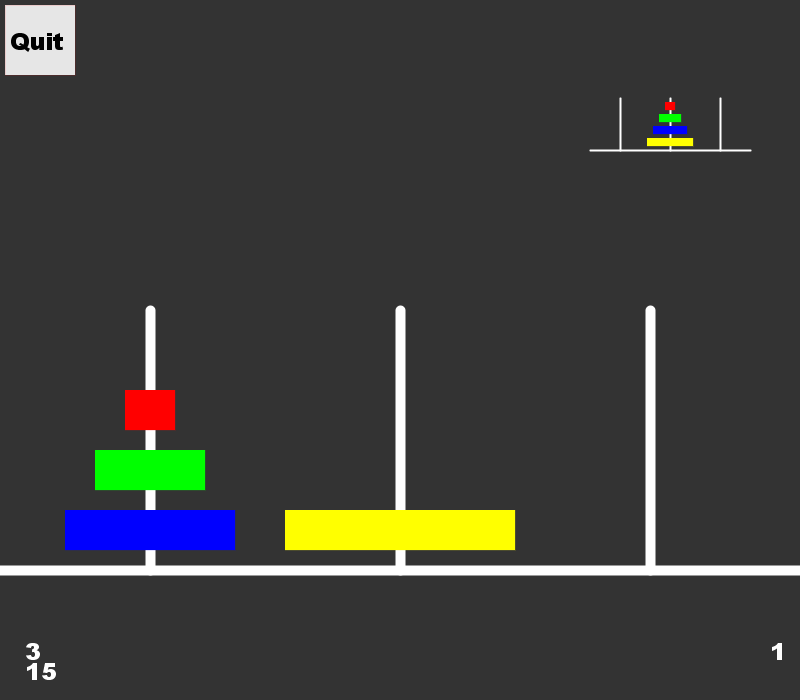
\includegraphics[height=.9\textheight]{towersofhanoi.png}}
\end{frame}

\begin{frame}{Towers of Hanoi}
  \begin{itemize}
  \item Rich mathematical tradition (state space = \alert{Sierpinski triangle}, optimal solution for 4 pegs still open);
  \item Classic algorithmic problem in computer science - shortest path algorithm recursively defined (variant of \alert{Dijkstra's algorithm} - dynamic programming);
  \item Popular task in \alert{developmental psychology} for assessing \emph{executive function} (attention, planning, etc).
  \end{itemize}
\end{frame}

\begin{frame}{Towers of Hanoi}
\centerline{
 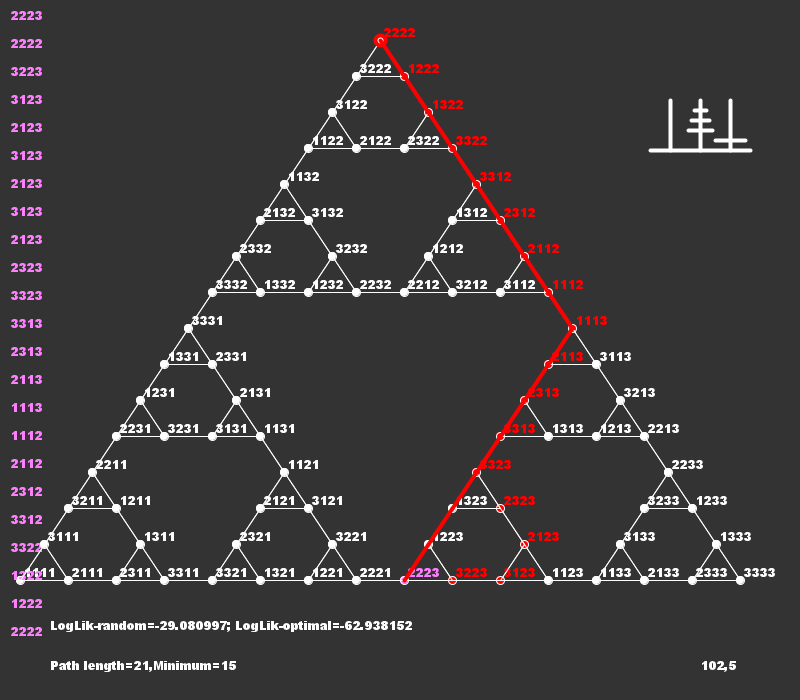
\includegraphics[height=.9\textheight]{toh.png}}
\end{frame}

\begin{frame}{Observation}
  Errors reveal much about the strategy used
\end{frame}

\section{Analysis}
\label{sec:analysis}

\begin{frame}{Shortest paths}
\centerline{
 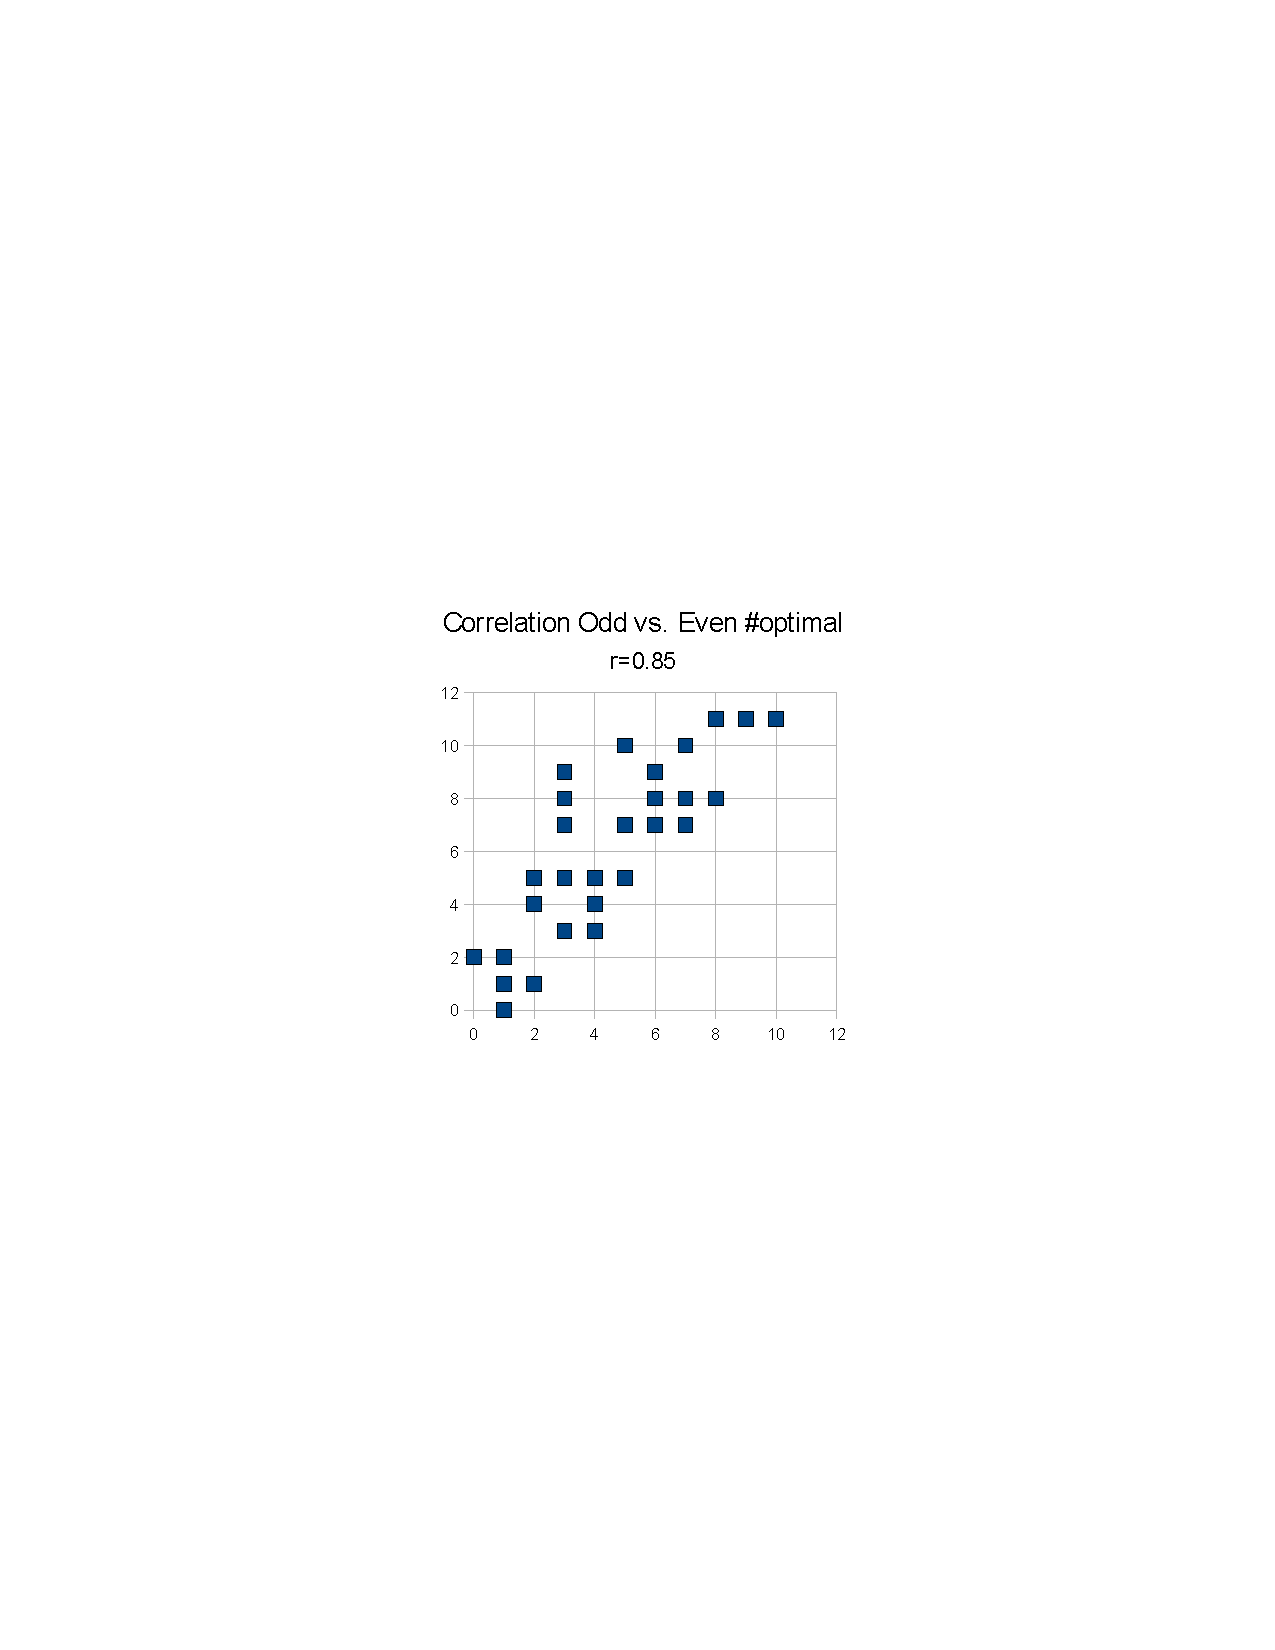
\includegraphics[trim= 10cm 10cm 10cm 10cm,height=.9\textheight]{numbershortest.pdf}}
\end{frame}

\begin{frame}{Shortest paths}
\centerline{
 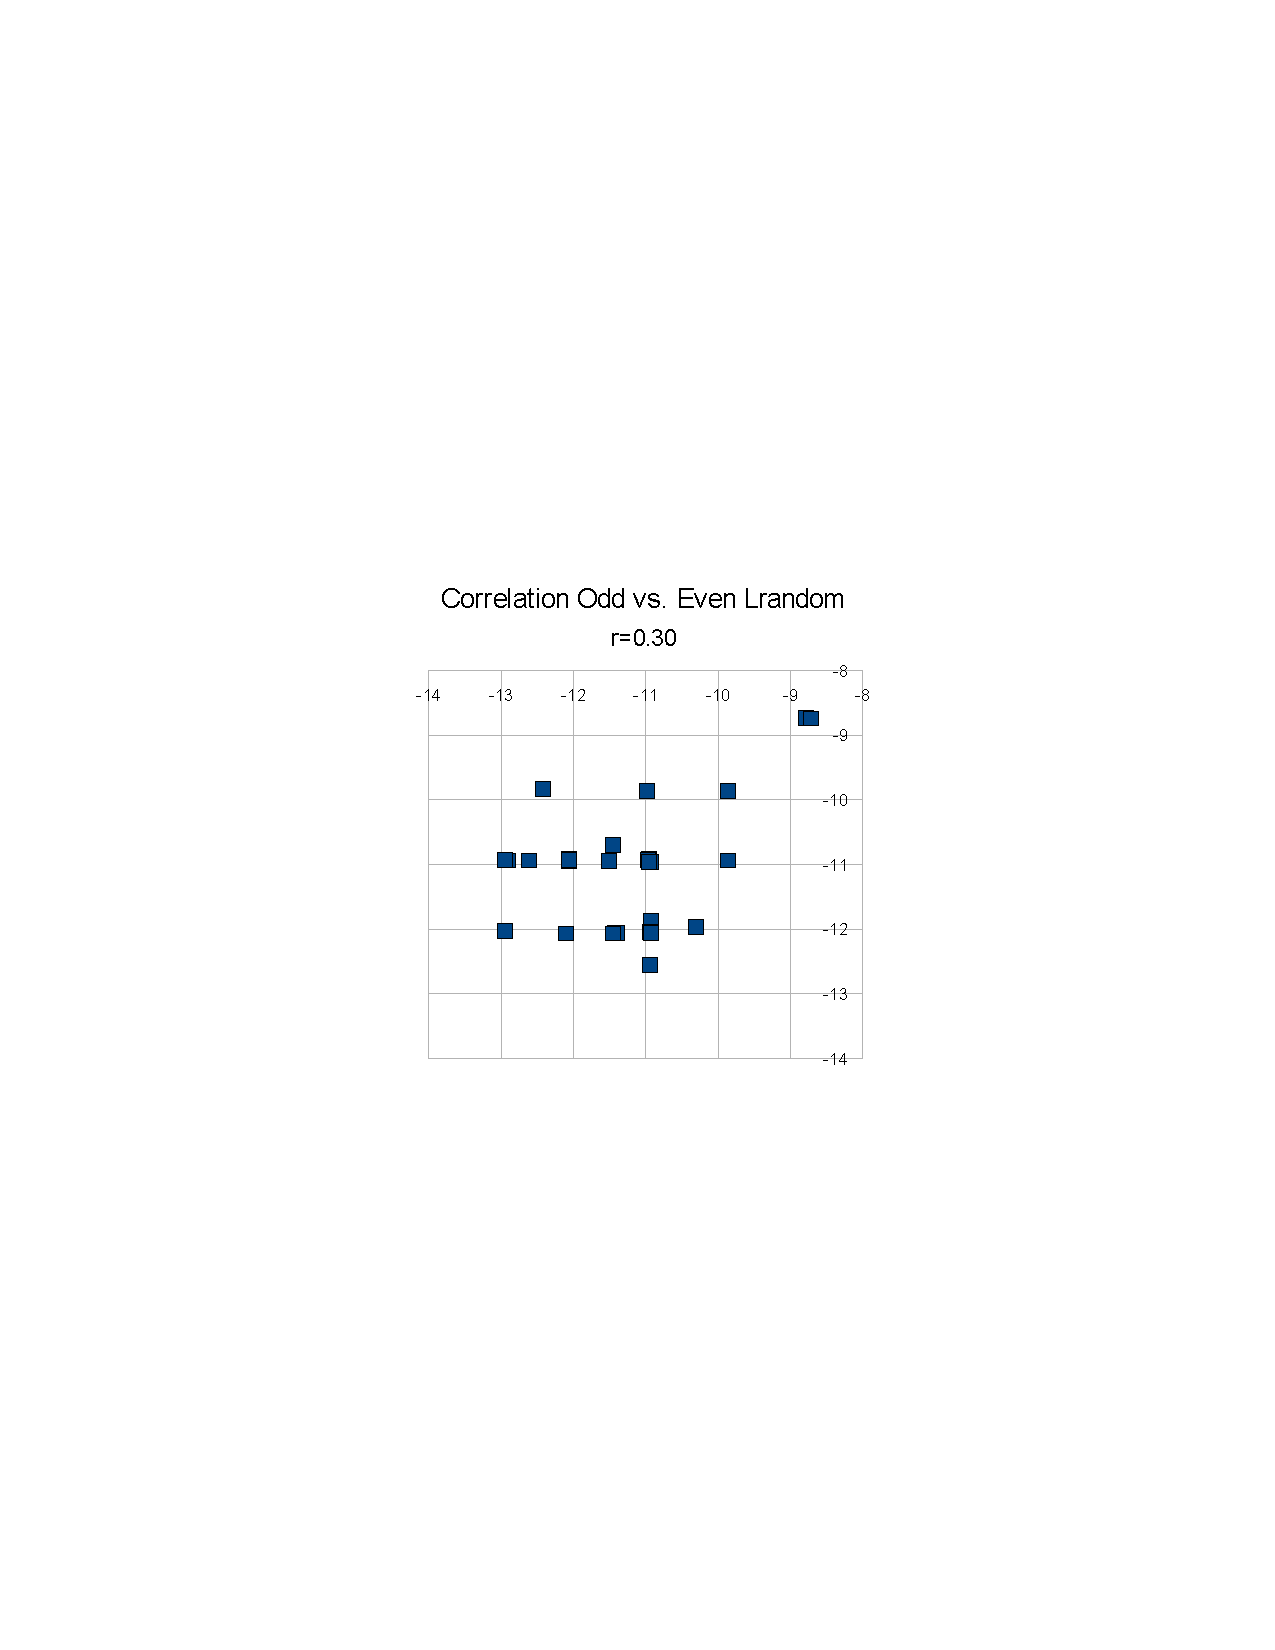
\includegraphics[trim= 10cm 10cm 10cm 10cm,height=.9\textheight]{lrandom.pdf}}
\end{frame}

\begin{frame}{Shortest paths}
\centerline{
 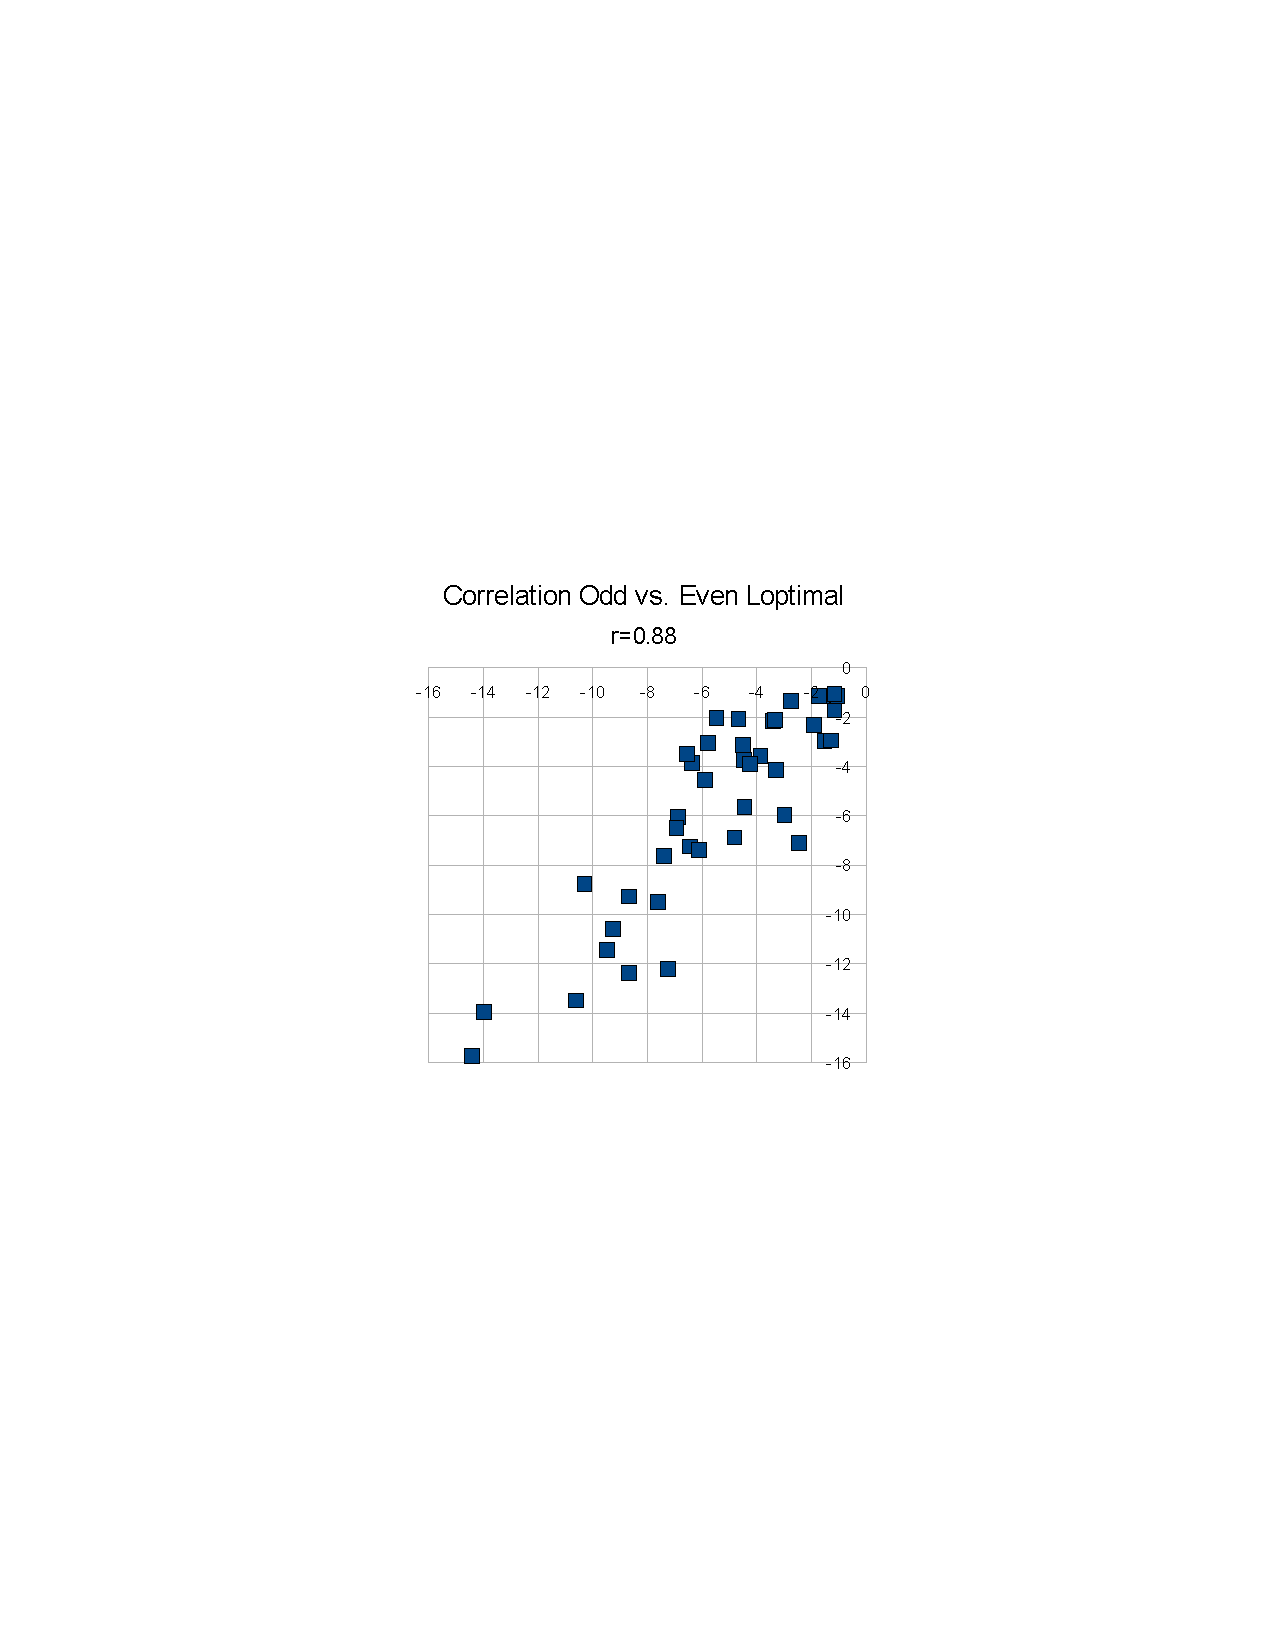
\includegraphics[trim= 10cm 10cm 10cm 10cm,height=.9\textheight]{loptimal.pdf}}
\end{frame}

\begin{frame}{Shortest paths}
\centerline{
 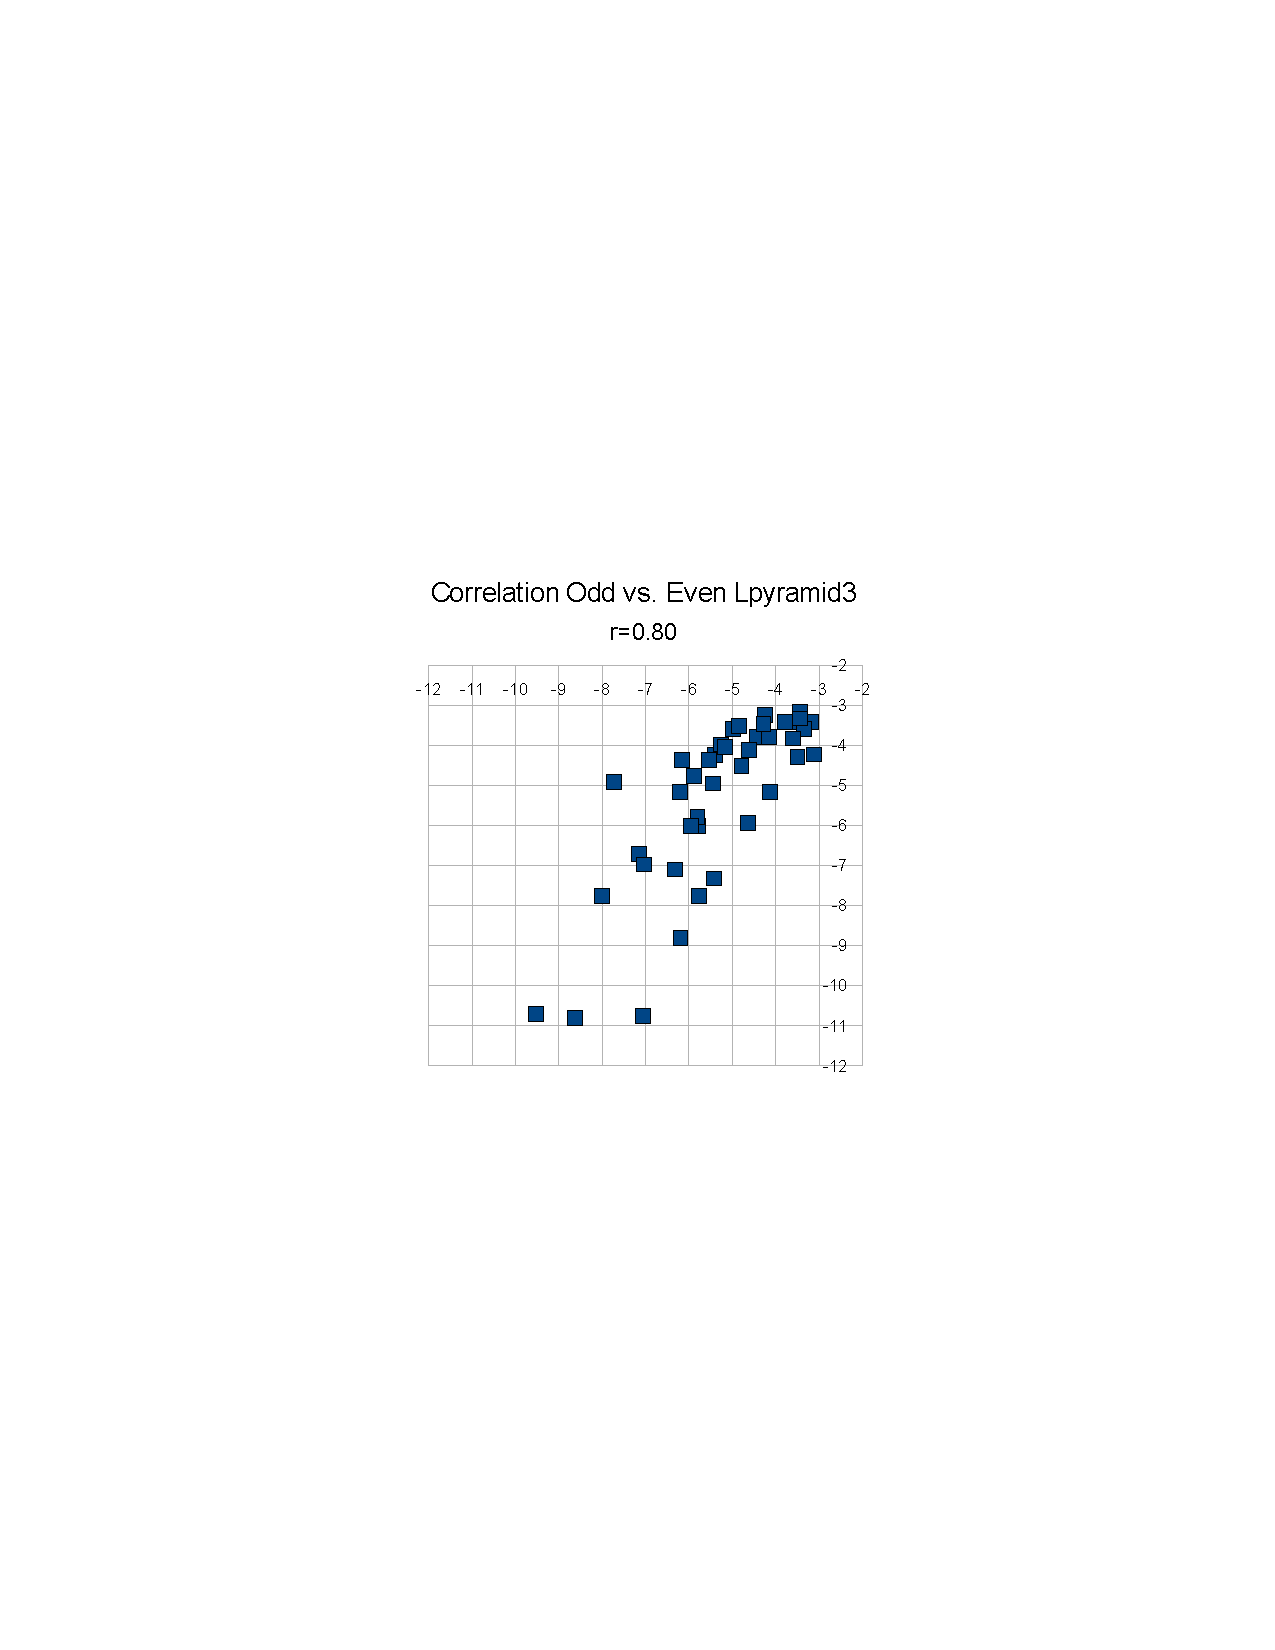
\includegraphics[trim= 10cm 10cm 10cm 10cm,height=.9\textheight]{lpyramid3.pdf}}
\end{frame}


\section{Conclusions}
\label{sec:conclusions}

\begin{frame}
  this analysis of the Tower of Hanoi problem may serve as a warning,
  illustrating the diversity of behavior that may be hidden under a
  blanket label like ``problem-solution process'' even in a very
  simple task environment. If we are to understand human
  problem-solving behavior, we must get a solid grip on the strategies
  that underlie that behavior, and we must avoid blending together in
  a statistical stew quite diverse problem solving behaviors whose
  real significance is lost in the averaging process. -- Herbert Simon
  (1975, p288)
\end{frame}



\begin{frame}{Recursion}

  \begin{itemize}[<+->]
  \item Major debate in linguistics and cognitive science about
    \begin{itemize}[<+->]
    \item 
    whether recursion is a fundamental property of language,
  \item whether
    it is a property of all human languages, and
  \item whether it is the
    only cognitive mechanism unique to language,
  \item and thus the core component of an innate Universal Grammar.
    \end{itemize}
  \item Is there is empirical data in (child) language corpora relevant to this debate?
  \end{itemize}

\end{frame}

\begin{frame}{Newspaper text}

  \begin{columns}
\column[t]{.5\textwidth}
\Tree [.{\only<2->{\color{red}}S} [.NP Mary ] [.VP [.V knows ] [.{\only<2->{\color{red}}S} [.NP John ] [.VP [.V lies ] ]]]] 
\column[t]{.5\textwidth}
\begin{itemize}[<+->]
\item Penn WSJ corpus: 30,000 sentences annotated with phrase-structure
\item<2-> Recursion: phrases of category X embedded in a phrase of same category X
\item<3-> Y \emph{dominates} X: a phrase of category X is embedded in a phrase of category Y
\end{itemize}
  \end{columns}
\end{frame}

\begin{frame}{Dominance matrix}
\centerline{\resizebox{1.2\linewidth}{!}{
  \begin{tabular}[t]{l|ccccccccc}
& \multicolumn{9}{c}{\emph{category of dominating node}}\\
 & S & VP & NP & TOP & PP & SBAR & SINV & ADJP & ADVP\\ \hline
S & \only<2>{\y} 82439 & \only<3->{\w}84506 & \only<3->{\w}23217 & \only<3->{\w}90756 & \only<3->{\w}13475 & \only<3->{\w}41930 & \only<3->{\w}5157 & \only<3->{\w}2415 & \only<3->{\w}353\\
VP & 255457 & \only<2>{\y} 186039 & \only<3->{\w}43154 & \only<3->{\w}132721 & \only<3->{\w}22915 & \only<3->{\w}64418 & \only<3->{\w}7546 & \only<3->{\w}4300 & \only<3->{\w}521\\
NP & 541368 & 521562 & \only<2>{\y} 279264 & \only<3->{\w} 318194 & \only<3->{\w}201943 & \only<3->{\w}123705 & \only<3->{\w}18139 & \only<3->{\w}11418 & \only<3->{\w}4726\\
TOP & 0 & 0 & 0 & \only<2>{\y} 0 & \only<3->{\w}0 & \only<3->{\w}0 & \only<3->{\w}0 & \only<3->{\w}0 & \only<3->{\w}0\\
PP & 144336 & 167814 & 80558 & 86865 & \only<2>{\y} 35679 & \only<3->{\w}32068 & \only<3->{\w}4184 & \only<3->{\w}4578 & \only<3->{\w}1690\\
SBAR & 40041 & 42621 & 15599 & 27749 & 7000 & \only<2>{\y} 6795 & \only<3->{\w}1616 & \only<3->{\w}991 & \only<3->{\w}264\\
SINV & 265 & 182 & 31 & 1834 & 10 & 106 & \only<2>{\y} 26 & \only<3->{\w}9 & \only<3->{\w}1\\
ADJP & 23600 & 25107 & 12813 & 13241 & 4610 & 5640 & 745 & \only<2>{\y} 1368 & \only<3->{\w}87\\
ADVP & 35876 & 36586 & 7728 & 20385 & 5005 & 9647 & 1056 & 659 & \only<2>{\y} 629
  \end{tabular}}}

\vfill

\only<4->{\alert{Category promiscuity!}}
~

\end{frame}


  \begin{frame}{Child language (2;3-2;11)}
\centerline{\resizebox{1.2\linewidth}{!}{    \begin{tabular}[t]{ccccccccccc}
       &  TOP &  COMP &  XCOMP &  LOC &  CJCT &  PRED &  COM &  PTL &  OBJ2 &  SRL\\
 TOP & 0 & 0 & 0 & 0 & 0 & 0 & 0 & 0 & 0 & 0\\
 COMP & 172 & 23 & 0 & 0 & 0 & 0 & 0 & 0 & 0 & 0\\
 XCOMP & 230 & 8 & 40 & 0 & 0 & 0 & 0 & 0 & 0 & 0\\
 LOC & 77 & 1 & 1 & 0 & 0 & 0 & 0 & 0 & 0 & 0\\
 CJCT & 10 & 3 & 0 & 0 & 1 & 0 & 0 & 0 & 0 & 0\\
 PRED & 61 & 0 & 0 & 0 & 1 & 0 & 0 & 0 & 0 & 0\\
 COM & 9 & 0 & 0 & 0 & 0 & 0 & 2 & 0 & 0 & 0\\
 PTL & 1 & 0 & 0 & 0 & 0 & 0 & 0 & 0 & 0 & 0\\
 OBJ2 & 24 & 0 & 0 & 0 & 0 & 0 & 0 & 0 & 0 & 0\\
 SRL & 17 & 0 & 0 & 0 & 0 & 0 & 0 & 0 & 0 & 1
    \end{tabular}}}
  \end{frame}

  \begin{frame}{Child language (3;6-4;5)}
\centerline{\resizebox{1.2\linewidth}{!}{    
\begin{tabular}[t]{ccccccccccc}
TOP &  COMP &  XCOMP &  PRED &  COORD &  JCT &  LOC &  CJCT &  OBJ &  SUBJ\\
515 & 92 & 14 & 0 & 12 & 1 & 0 & 0 & 0 & 0\\
855 & 56 & 33 & 12 & 19 & 0 & 0 & 4 & 1 & 1\\
782 & 40 & 31 & 4 & 25 & 0 & 0 & 6 & 1 & 1\\
423 & 7 & 30 & 7 & 23 & 12 & 0 & 3 & 26 & 2\\
1142 & 75 & 195 & 24 & 60 & 5 & 2 & 7 & 21 & 13\\
154 & 13 & 30 & 3 & 8 & 0 & 0 & 0 & 0 & 0\\
88 & 11 & 8 & 1 & 1 & 0 & 0 & 0 & 0 & 0\\
1433 & 92 & 187 & 19 & 57 & 4 & 0 & 22 & 8 & 4\\
570 & 41 & 8 & 4 & 27 & 4 & 0 & 3 & 0 & 9
    \end{tabular}}}
  \end{frame}


\end{document}
%---------------------------------------------------------------------------------------

% Opportunity to present my view on research at ILLC

% Many problems in cognitive science demand collaboration between modellers and experimentalists
% Modellers that go at it alone
% Experimentalists that go at it alone 
% Models need crosschecking with other models and experimental data - e.g., Gold's proof
% ILLC is in a unique position to fulfill that role
